% Options for packages loaded elsewhere
\PassOptionsToPackage{unicode}{hyperref}
\PassOptionsToPackage{hyphens}{url}
%
\documentclass[
]{article}
\usepackage{lmodern}
\usepackage{amssymb,amsmath}
\usepackage{ifxetex,ifluatex}
\ifnum 0\ifxetex 1\fi\ifluatex 1\fi=0 % if pdftex
  \usepackage[T1]{fontenc}
  \usepackage[utf8]{inputenc}
  \usepackage{textcomp} % provide euro and other symbols
\else % if luatex or xetex
  \usepackage{unicode-math}
  \defaultfontfeatures{Scale=MatchLowercase}
  \defaultfontfeatures[\rmfamily]{Ligatures=TeX,Scale=1}
\fi
% Use upquote if available, for straight quotes in verbatim environments
\IfFileExists{upquote.sty}{\usepackage{upquote}}{}
\IfFileExists{microtype.sty}{% use microtype if available
  \usepackage[]{microtype}
  \UseMicrotypeSet[protrusion]{basicmath} % disable protrusion for tt fonts
}{}
\makeatletter
\@ifundefined{KOMAClassName}{% if non-KOMA class
  \IfFileExists{parskip.sty}{%
    \usepackage{parskip}
  }{% else
    \setlength{\parindent}{0pt}
    \setlength{\parskip}{6pt plus 2pt minus 1pt}}
}{% if KOMA class
  \KOMAoptions{parskip=half}}
\makeatother
\usepackage{xcolor}
\IfFileExists{xurl.sty}{\usepackage{xurl}}{} % add URL line breaks if available
\IfFileExists{bookmark.sty}{\usepackage{bookmark}}{\usepackage{hyperref}}
\hypersetup{
  pdftitle={Delay reasons for TTC in May 2020},
  pdfauthor={Junjie Peng},
  hidelinks,
  pdfcreator={LaTeX via pandoc}}
\urlstyle{same} % disable monospaced font for URLs
\usepackage[margin=1in]{geometry}
\usepackage{color}
\usepackage{fancyvrb}
\newcommand{\VerbBar}{|}
\newcommand{\VERB}{\Verb[commandchars=\\\{\}]}
\DefineVerbatimEnvironment{Highlighting}{Verbatim}{commandchars=\\\{\}}
% Add ',fontsize=\small' for more characters per line
\usepackage{framed}
\definecolor{shadecolor}{RGB}{248,248,248}
\newenvironment{Shaded}{\begin{snugshade}}{\end{snugshade}}
\newcommand{\AlertTok}[1]{\textcolor[rgb]{0.94,0.16,0.16}{#1}}
\newcommand{\AnnotationTok}[1]{\textcolor[rgb]{0.56,0.35,0.01}{\textbf{\textit{#1}}}}
\newcommand{\AttributeTok}[1]{\textcolor[rgb]{0.77,0.63,0.00}{#1}}
\newcommand{\BaseNTok}[1]{\textcolor[rgb]{0.00,0.00,0.81}{#1}}
\newcommand{\BuiltInTok}[1]{#1}
\newcommand{\CharTok}[1]{\textcolor[rgb]{0.31,0.60,0.02}{#1}}
\newcommand{\CommentTok}[1]{\textcolor[rgb]{0.56,0.35,0.01}{\textit{#1}}}
\newcommand{\CommentVarTok}[1]{\textcolor[rgb]{0.56,0.35,0.01}{\textbf{\textit{#1}}}}
\newcommand{\ConstantTok}[1]{\textcolor[rgb]{0.00,0.00,0.00}{#1}}
\newcommand{\ControlFlowTok}[1]{\textcolor[rgb]{0.13,0.29,0.53}{\textbf{#1}}}
\newcommand{\DataTypeTok}[1]{\textcolor[rgb]{0.13,0.29,0.53}{#1}}
\newcommand{\DecValTok}[1]{\textcolor[rgb]{0.00,0.00,0.81}{#1}}
\newcommand{\DocumentationTok}[1]{\textcolor[rgb]{0.56,0.35,0.01}{\textbf{\textit{#1}}}}
\newcommand{\ErrorTok}[1]{\textcolor[rgb]{0.64,0.00,0.00}{\textbf{#1}}}
\newcommand{\ExtensionTok}[1]{#1}
\newcommand{\FloatTok}[1]{\textcolor[rgb]{0.00,0.00,0.81}{#1}}
\newcommand{\FunctionTok}[1]{\textcolor[rgb]{0.00,0.00,0.00}{#1}}
\newcommand{\ImportTok}[1]{#1}
\newcommand{\InformationTok}[1]{\textcolor[rgb]{0.56,0.35,0.01}{\textbf{\textit{#1}}}}
\newcommand{\KeywordTok}[1]{\textcolor[rgb]{0.13,0.29,0.53}{\textbf{#1}}}
\newcommand{\NormalTok}[1]{#1}
\newcommand{\OperatorTok}[1]{\textcolor[rgb]{0.81,0.36,0.00}{\textbf{#1}}}
\newcommand{\OtherTok}[1]{\textcolor[rgb]{0.56,0.35,0.01}{#1}}
\newcommand{\PreprocessorTok}[1]{\textcolor[rgb]{0.56,0.35,0.01}{\textit{#1}}}
\newcommand{\RegionMarkerTok}[1]{#1}
\newcommand{\SpecialCharTok}[1]{\textcolor[rgb]{0.00,0.00,0.00}{#1}}
\newcommand{\SpecialStringTok}[1]{\textcolor[rgb]{0.31,0.60,0.02}{#1}}
\newcommand{\StringTok}[1]{\textcolor[rgb]{0.31,0.60,0.02}{#1}}
\newcommand{\VariableTok}[1]{\textcolor[rgb]{0.00,0.00,0.00}{#1}}
\newcommand{\VerbatimStringTok}[1]{\textcolor[rgb]{0.31,0.60,0.02}{#1}}
\newcommand{\WarningTok}[1]{\textcolor[rgb]{0.56,0.35,0.01}{\textbf{\textit{#1}}}}
\usepackage{graphicx,grffile}
\makeatletter
\def\maxwidth{\ifdim\Gin@nat@width>\linewidth\linewidth\else\Gin@nat@width\fi}
\def\maxheight{\ifdim\Gin@nat@height>\textheight\textheight\else\Gin@nat@height\fi}
\makeatother
% Scale images if necessary, so that they will not overflow the page
% margins by default, and it is still possible to overwrite the defaults
% using explicit options in \includegraphics[width, height, ...]{}
\setkeys{Gin}{width=\maxwidth,height=\maxheight,keepaspectratio}
% Set default figure placement to htbp
\makeatletter
\def\fps@figure{htbp}
\makeatother
\setlength{\emergencystretch}{3em} % prevent overfull lines
\providecommand{\tightlist}{%
  \setlength{\itemsep}{0pt}\setlength{\parskip}{0pt}}
\setcounter{secnumdepth}{-\maxdimen} % remove section numbering

\title{Delay reasons for TTC in May 2020}
\author{Junjie Peng}
\date{2020/9/27}

\begin{document}
\maketitle
\begin{abstract}
The public transportations are convenient and low carbon, but the
problem of bus delays is troubling.In this study, we explored the bus
delay data provided by THE TTC and found that the main reason for bus
delay in May 2020 were mechanical problem and Utilized off Route.Our
findings may help reduce the problem of bus delays.
\end{abstract}

\hypertarget{introduction}{%
\section{Introduction}\label{introduction}}

Public transport is an important part of daily life. Compared with other
modes of transport, it has advantages such as low cost and low carbon
emissions.But it also has some disadvantages, for example, the problem
that the bus is late is very disturbing.Long waits are likely to disrupt
travelers' plans, with unpleasant results.Therefore, this study intends
to briefly explore the main reasons for bus delay and some improvement
methods from the data of bus delay provided by TTC.

To ensure the timeliness of the data, the study only selected data from
May 2020.Among the many categories provided by the data, only the
reasons for the delay were selected for study.Although there may be a
lot of distractions associated with such a choice, the purpose of this
study is to provide a simple and intuitive understanding of the causes
of bus delays, so this study has some significance for those who do not
know the public transport system.The following content will show the
code of data extraction and the bar chart of the reason of bus delay,
followed by the discussion of the data results and the reflection on the
research itself.

\begin{Shaded}
\begin{Highlighting}[]
\KeywordTok{library}\NormalTok{(opendatatoronto)}
\KeywordTok{library}\NormalTok{(dplyr)}
\KeywordTok{library}\NormalTok{(ggplot2)}
\end{Highlighting}
\end{Shaded}

\begin{Shaded}
\begin{Highlighting}[]
\CommentTok{# get package for TTC delay data}
\KeywordTok{list_package_resources}\NormalTok{(}\StringTok{"e271cdae-8788-4980-96ce-6a5c95bc6618"}\NormalTok{)}
\end{Highlighting}
\end{Shaded}

\begin{verbatim}
## # A tibble: 8 x 4
##   name                     id                               format last_modified
##   <chr>                    <chr>                            <chr>  <date>       
## 1 ttc-bus-delay-data-read~ fed6d76e-9167-4268-9eb1-139fcde~ XLSX   2019-08-15   
## 2 ttc-bus-delay-data-2014  86fb9e42-5b92-4473-8f59-9d2af4f~ XLSX   2019-08-15   
## 3 ttc-bus-delay-data-2015  e7167258-71e4-47f6-9fe3-2b942e3~ XLSX   2019-08-15   
## 4 ttc-bus-delay-data-2016  db758903-72b5-4df2-a582-0a1be6e~ XLSX   2019-08-15   
## 5 ttc-bus-delay-data-2017  d0dd6840-4eda-4a1f-8d06-454d11e~ XLSX   2019-08-15   
## 6 ttc-bus-delay-data-2018  adb41bd4-9869-4f50-96e6-5e881b9~ XLSX   2019-08-15   
## 7 ttc-bus-delay-data-2019  e2ee1c1c-9839-45a6-9345-57084e3~ XLSX   2020-04-28   
## 8 ttc-bus-delay-data-2020  fac1d636-8158-47ec-bfa2-01bc7d0~ XLSX   2020-06-22
\end{verbatim}

\begin{Shaded}
\begin{Highlighting}[]
\CommentTok{# get package for TTC delay data in May 2020}
\NormalTok{TTC_delay_}\DecValTok{2020}\NormalTok{ <-}\StringTok{ }\KeywordTok{get_resource}\NormalTok{(}\StringTok{"fac1d636-8158-47ec-bfa2-01bc7d061f46"}\NormalTok{)}
\NormalTok{TTC_delay_}\DecValTok{2020}\OperatorTok{$}\StringTok{`}\DataTypeTok{May 2020}\StringTok{`}
\end{Highlighting}
\end{Shaded}

\begin{verbatim}
## # A tibble: 3,504 x 10
##    `Report Date`       Route Time                Day   Location Incident Delay
##    <dttm>              <dbl> <dttm>              <chr> <chr>    <chr>    <dbl>
##  1 2020-05-01 00:00:00   329 1899-12-31 01:31:00 Frid~ STEELES~ Mechani~    30
##  2 2020-05-01 00:00:00   300 1899-12-31 03:20:00 Frid~ The Wes~ Emergen~     3
##  3 2020-05-01 00:00:00    35 1899-12-31 04:04:00 Frid~ PVST     Late Le~     1
##  4 2020-05-01 00:00:00   600 1899-12-31 05:00:00 Frid~ Eglinto~ Utilize~     1
##  5 2020-05-01 00:00:00   600 1899-12-31 05:00:00 Frid~ Eglinto~ Utilize~     1
##  6 2020-05-01 00:00:00    63 1899-12-31 05:31:00 Frid~ King/At~ Utilize~    13
##  7 2020-05-01 00:00:00    50 1899-12-31 05:46:00 Frid~ Mill lo~ Late Le~     1
##  8 2020-05-01 00:00:00   129 1899-12-31 06:00:00 Frid~ STC      Late Le~     6
##  9 2020-05-01 00:00:00   116 1899-12-31 06:05:00 Frid~ Kennedy  Late Le~    17
## 10 2020-05-01 00:00:00    12 1899-12-31 06:09:00 Frid~ Brimley~ Investi~    13
## # ... with 3,494 more rows, and 3 more variables: Gap <dbl>, Direction <chr>,
## #   Vehicle <dbl>
\end{verbatim}

\hypertarget{plots}{%
\section{Plots}\label{plots}}

\begin{Shaded}
\begin{Highlighting}[]
\KeywordTok{ggplot}\NormalTok{(TTC_delay_}\DecValTok{2020}\OperatorTok{$}\StringTok{`}\DataTypeTok{May 2020}\StringTok{`}\NormalTok{, }\KeywordTok{aes}\NormalTok{(}\DataTypeTok{x=}\NormalTok{Incident)) }\OperatorTok{+}\StringTok{ }\KeywordTok{geom_bar}\NormalTok{() }\OperatorTok{+}\StringTok{ }
\StringTok{  }\KeywordTok{theme}\NormalTok{(}\DataTypeTok{axis.text.x =} \KeywordTok{element_text}\NormalTok{(}\DataTypeTok{angle =} \DecValTok{30}\NormalTok{, }\DataTypeTok{hjust =} \DecValTok{1}\NormalTok{))}
\end{Highlighting}
\end{Shaded}

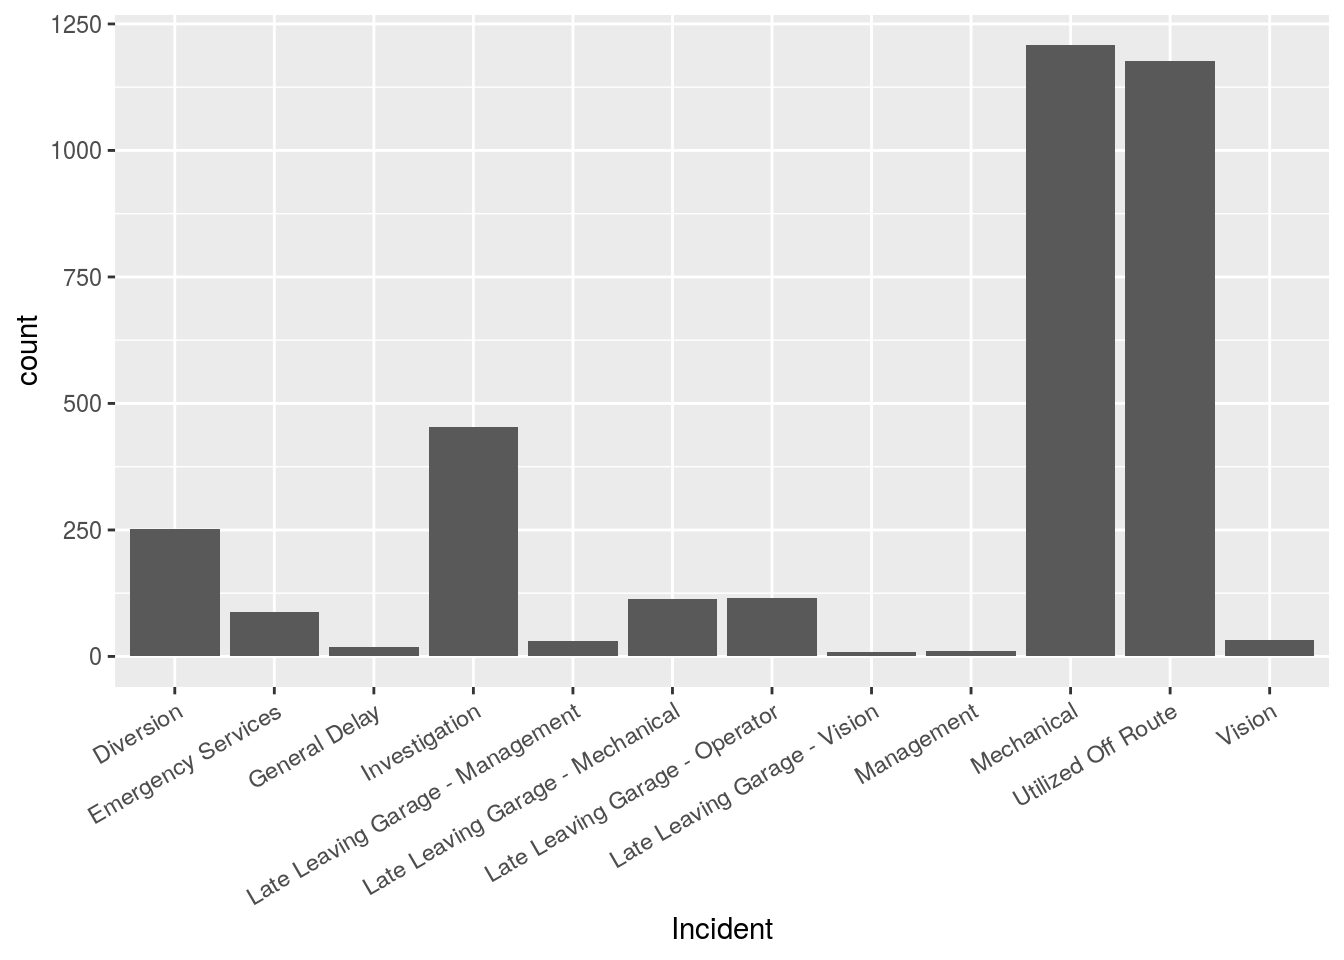
\includegraphics{test_files/figure-latex/unnamed-chunk-3-1.pdf}

\hypertarget{discussion}{%
\section{Discussion}\label{discussion}}

From the histgram it is easily to find out that there are two main
reasons for the delay of TTC in May 2020, which are `Mechanical' and
`Utilized off Route'.Therefore, in order to decrease the time of delay
the TTC could focous on these two aspects. To be more specific, for the
mechanical problems, it seems inevitable, but periodic maintenance of
equipment and vehicles should effectively reduce the occurrence of
problems. For the incident of `Utilized off Route',To be honest, I have
no idea about the management of public transportation system, so I can
only make a simple conjecture here.This may be a problem caused by
improper vehicle routing, so a proper route planning may reduce the
occurrence of accidents.For example, try to avoid a large number of
routes overlap, or when the need to dispatch vehicles to pick up a
number of idle shifts, etc.

\hypertarget{weaknesses-and-future-directions}{%
\section{Weaknesses and future
directions}\label{weaknesses-and-future-directions}}

Objectively speaking, this simple study has many problems and needs to
be improved.First of all, the sample size I selected is very small, just
the data of May 2020.We know that 2020 is a very special year, and the
way we use public transport in the event of quarantine may be very
different from what we used to be, that's something that this study
didn't take into account.Secondly, this data includes a large number of
sites and regions, but the differences among different regions are not
taken into account in the study of the reasons for delay, because the
distribution of these reasons is likely to be uneven. The two main
reasons mentioned above may be clustered in a specific small range
rather than common reasons in general.Therefore, in further studies,
time and regional differences should be taken into account, so that such
results will be more convincing.

\hypertarget{reference}{%
\section{Reference}\label{reference}}

\begin{itemize}
\tightlist
\item
  Sharla Gelfand (2020). opendatatoronto: Access the City of Toronto
  Open Data Portal. R package version 0.1.3.
  \url{https://CRAN.R-project.org/package=opendatatoronto}
\item
  Hadley Wickham, Romain François, Lionel Henry and Kirill Müller
  (2020). dplyr: A Grammar of Data Manipulation. R package version
  1.0.0. \url{https://CRAN.R-project.org/package=dplyr}
\item
  H. Wickham. ggplot2: Elegant Graphics for Data Analysis.
  Springer-Verlag New York, 2016.
\item
  R Core Team (2019). R: A language and environment for statistical
  computing. R Foundation for Statistical Computing, Vienna, Austria.
  URL \url{https://www.R-project.org/}.
\item
  Toronto Transit Commission(2020). TTC Bus Delay Data.opendatatoronto:
  Access the City of Toronto Open Data
  Portal.https://open.toronto.ca/dataset/ttc-bus-delay-data/
\end{itemize}

\end{document}
